%%%%%%%%%%%%%%%%%%%%%%%%%%%%%%%%%%%%%%%%%%%%%%%
%
%   Results
%
%%%%%%%%%%%%%%%%%%%%%%%%%%%%%%%%%%%%%%%%%%%%%%%

\subsection{Influence of Pool Size and Selection Size} \label{p-size.s-size}
\textbf{To answer} $\pmb{Q_5}$, we analyze how ordered aggregation is affected by both the initial pool size ($T$) and the selection percentage ($P$) simultaneously. A heterogeneous ensemble, see Section \ref{ch6_setup}, composed of 201 models is built. The classifiers will be ordered considering only the first 25, 51, 75, 101, 151, and 201 models from ensemble size. This means that the classifiers are nested such that all classifiers in an initial pool are also included in larger pools. The average accuracy over 100 runs is computed for each ensemble size $T$. 

Table \ref{SpectfAcc} shows the analysis of 1200 records ($T=6$ $\times$ runs=100 $\times$ $P=2$) for the \textit{SPECTF} dataset. The last two columns represent the size of the ordered subensemble according to an initial pool of $T$. For each $T$ and $P$, the best value is highlighted in bold. The prediction accuracy of the bagging increases monotonically as a function of the initial pool size, while this saturation level sometimes decreases according to the classification task. All the investigated metrics prove their superiority over bagging, \textit{regarding SPECTF dataset}. The poor results reported for BSM, confirm that ensemble outperforms all single models from which it is composed. Regarding the selection percentage of $P=30\%$, the accuracy of DISC, EPIC, and UMEP keep on increasing as more classifiers are included in the initial pool. \textit{In general}, the accuracy of the ordered classifiers with a percentage of 30\% is better than 20\%. In addition, the poorest accuracy by any ordering metric is better than the highest accuracy of bagging. The highest accuracy of 91.49 is reported by DISC using a subensemble composed of 61 classifiers, $\hat{T}$, instead of the 201 classifiers used by bagging. 


\begin{table*}[!ht]
\centering\scriptsize
\caption{The average accuracy of the subensemble related to a selection percentage ($P$) from an inital pool size ($T$);\textit{ SPECTF dataset}.}
\resizebox{\textwidth}{!}{\begin{tabular}{ccc|cccccccc|cc}
  \hline
  \multicolumn{1}{c}{$T$}   & \multicolumn{1}{c}{Bagging} &\multicolumn{1}{c}{ BSM}  &\multicolumn{1}{c}{ RE} & \multicolumn{1}{c}{CC} & \multicolumn{1}{c}{MDSQ} & \multicolumn{1}{c}{MRMR} & \multicolumn{1}{c}{DISC}& \multicolumn{1}{c}{EPIC} & \multicolumn{1}{c}{UMEP} & \multicolumn{1}{c}{MDEP}  & \multicolumn{1}{c}{$P$} & \multicolumn{1}{c}{$\hat{T}$} \\ 
  \hline   
\multirow{2}{*}{25} & \multirow{2}{*}{\textbf{84.73}} & \multirow{2}{*}{81.87}  & 86.73 & 86.21  & 87.23 & 86.43  & \textbf{88.43} & 86.49 & 86.65 & 86.77 &  20\% & 5 \\
&&& 87.66  & 87.11 & 88.18	& 87.19	 & \textbf{88.69} & 87.77 & 87.74	  & 87.71 &  30\% & 7 \\ \hline

\multirow{2}{*}{51} & \multirow{2}{*}{\textbf{85.27}} & \multirow{2}{*}{82.96}  & 89.22  & 88.41 & 89.91  & 88.35 & \textbf{90.41} & 89.65 & 89.54 & 89.72 &  20\% & 11 \\
&&& 88.97  & 88.54 & 89.82 & 88.62 & \textbf{90.49}  & 89.65 & 89.76	  & 89.80 & 30\% & 15 \\ \hline

\multirow{2}{*}{75} & \multirow{2}{*}{\textbf{85.48}} & \multirow{2}{*}{82.92}  &  88.89 & 88.80 & 90.24  & 88.12  & \textbf{91.10}  & 90.28 & 90.83 & 90.66	 &  20\% & 15 \\
&&& 88.80  & 88.94  & 89.69 & 88.20 & \textbf{90.89}  & 90.38 & 90.32 & 90.21	 & 30\% & 23 \\ \hline

\multirow{2}{*}{101} & \multirow{2}{*}{\textbf{85.85}} & \multirow{2}{*}{83.09}  & 89.08  & 89.06 & 89.90 & 87.77 & \textbf{91.21} & 90.56 & 90.22 & 90.44 &  20\% & 21\\
&&& 88.93  & 88.80  & 88.83 & 88.14 & \textbf{91.01} & 90.84  & 90.41 & 90.78  & 30\% & 31 \\ \hline    

\multirow{2}{*}{151} & \multirow{2}{*}{\textbf{85.82}} & \multirow{2}{*}{82.78}  & 89.18  & 88.89  &  89.29 & 88.54 & \textbf{91.09} & 90.58 & 90.59 & 90.44 & 20\% & 31\\
&&& 88.82  & 88.97  & 88.03 & 88.91  & \textbf{91.24}  & 90.64 & 90.78 & 90.70 & 30\%  & 45\\ \hline

\multirow{2}{*}{201} & \multirow{2}{*}{\textbf{85.84}} & \multirow{2}{*}{83.68}  &  89.12 & 89.19 & 88.48  & 88.82 & 91.07  & 91.07  & \textbf{91.15} & 91.10	 & 20\% & 41 \\
&&& 89.22  & 88.88  & 87.36  & 88.70 & \textbf{91.49} & 91.00	 & 91.04 & 91.09 & 30\% & 61\\ \hline 
   
\end{tabular}}
\label{SpectfAcc}
\end{table*}

\begin{figure*}[!ht]
\centering
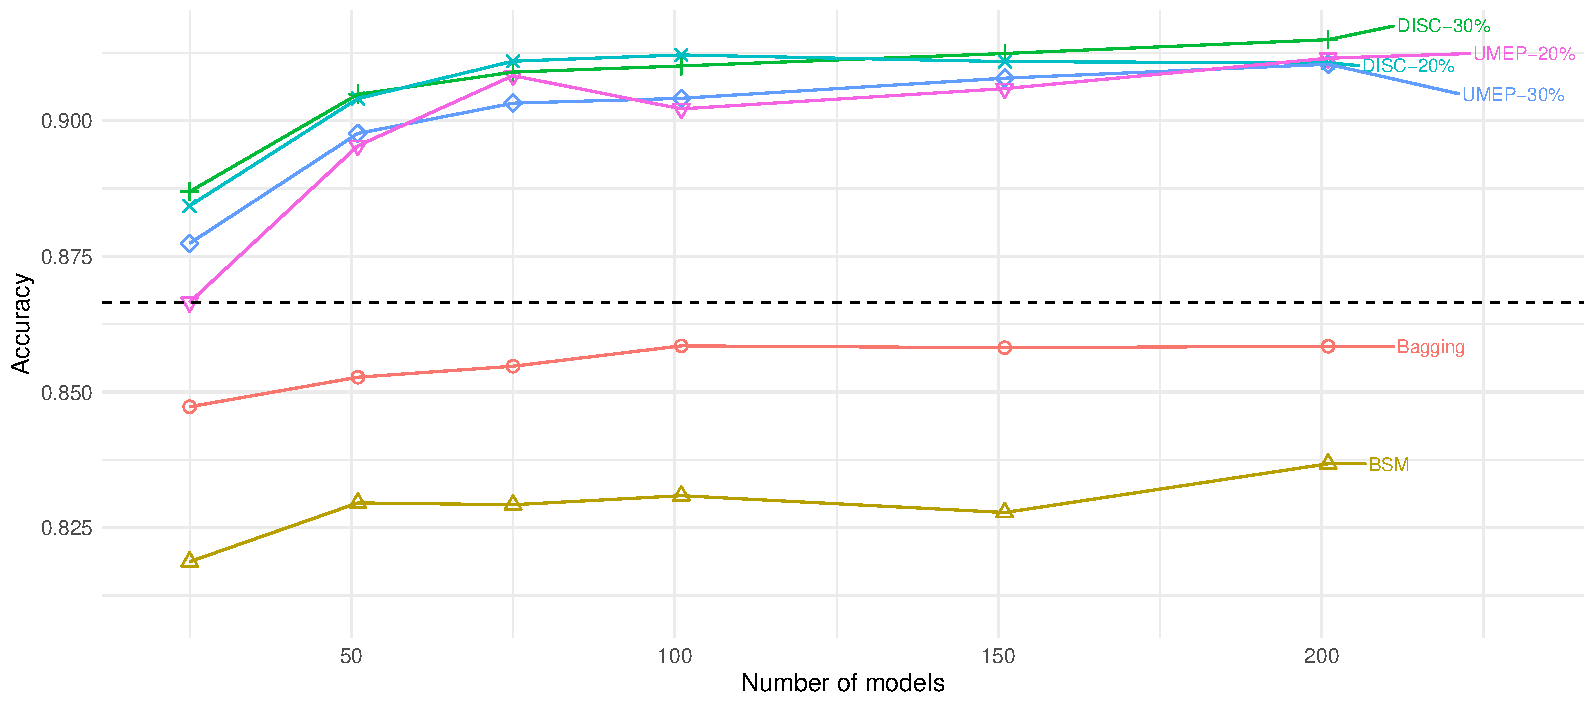
\includegraphics[width=1\textwidth]{6_analysis/fig/Selection.pdf}
\caption{Influence of pool size and selection size on the general accuracy; \textit{SPECTF dataset}.}
\label{Selection-size}
\end{figure*}




Figure \ref{Selection-size} shows the complementary perspective about the results. The comparison of DISC-30\% with DISC-20\% and the comparison of UMEP-30\% with UMEP-20\% confirm that the ordered subset with a larger number of classifiers returns higher accuracy. Furthermore, the lowest accuracy by UMEP-20\%, \textit{horizontal-dashed line}, with only 5 classifiers outperforms the accuracy of bagging for any size. The prediction accuracy of DISC-30\% and UMEP-30\% keeps on increasing even after bagging has stabilized. In addition, the figure shows that BSM is the worst ensemble selection strategy. We confirm that the main objective of heuristic metrics is to return a subensemble with a reduced number of classifiers while keeping the accuracy unaffected. Going beyond the accuracy of the bagging is conditioned by the effectiveness to reorder the ensemble as we will discuss in Sections \ref{overbinary} and \ref{overmulti}.   



\subsection{Influence of Heterogeneous Classifiers} \label{heter.class}

\textbf{To answer} $\pmb{Q_6}$, we analyze how the general accuracy and the performance of the metrics are affected by the type of combined individual models. For that, the initial pool size is fixed with $T=101$ as a balance between accuracy and ensemble's complexity. Then the two types of ensembles, \textit{homogeneous and heterogeneous}, described in Section \ref{ch6_setup}, are constructed for comparison purposes. Table \ref{individual-types} presents the average accuracy and the standard deviation for the ensembles using different and similar individual classifiers over six representative datasets. 

\vspace*{.3cm}
\begin{table*}[!ht]
        \centering\scriptsize
\caption{Average accuracy and standard deviation for Different Classifiers (DC) and Similar Classifiers (SC); $T$= 101 and $P$=30\%.}
\label{individual-types}
\resizebox{\textwidth}{!}{\begin{tabular}{lcccc||cccc}
  \hline
 &  \multicolumn{4}{c}{DC}&\multicolumn{4}{c}{SC}\\
 \cmidrule(lr){2-5} \cmidrule(lr){6-9}
 
   Dataset   & \multicolumn{1}{c} {Bagging} & \multicolumn{1}{c} {RE} & \multicolumn{1}{c} {DISC} & \multicolumn{1}{c||} {UMEP} & \multicolumn{1}{c} {Bagging} & \multicolumn{1}{c} {RE} & \multicolumn{1}{c} {DISC} & \multicolumn{1}{c} {UMEP}   \\ 
\hline
Ensemble size&\multicolumn{1}{c|} {$T=101$} & \multicolumn{3}{c||} {$\hat{T}=31$} & \multicolumn{1}{c|}{$T=101$} & \multicolumn{3}{c} {$\hat{T}=31$} \\
   \hline
 Australian &  86.70 $\pm$ 3.39 & \textbf{86.97 $\pm$ 3.52} & \textbf{86.97 $\pm$ 3.48}  &  \textbf{87.36 $\pm$ 3.35} & 86.85 $\pm$ 3.43 & 86.66 $\pm$ 3.85  & 86.34 $\pm$ 3.81  & \textbf{86.95 $\pm$	3.67}   \\
 
Blood &  77.37 $\pm$ 1.77 & 77.35 $\pm$ 2.68 & \textbf{77.53 $\pm$ 2.74} & 77.03 $\pm$ 2.73& 76.27 $\pm$ 0.73 &\textbf{77.53 $\pm$ 2.77}  & \textbf{77.92 $\pm$ 2.47}  & \textbf{77.14 $\pm$ 2.80}	   \\
 
Breast-cancer & 73.41 $\pm$ 5.73 & \textbf{73.94 $\pm$ 6.84}  &  \textbf{73.45 $\pm$ 6.03} & 72.97 $\pm$ 6.90 & 73.48	 $\pm$ 	5.08  & 73.02 $\pm$ 5.63   & 73.10 $\pm$ 5.58& 71.41  $\pm$ 6.39 	   \\

Cmc & 53.30 $\pm$ 3.74 & 53.29 $\pm$ 3.83 & \textbf{53.80  $\pm$ 3.72}  & \textbf{53.82  $\pm$ 3.69} & 53.33 $\pm$ 3.84 & \textbf{53.38 $\pm$ 3.41} & \textbf{53.57 $\pm$ 3.58} & \textbf{53.65 $\pm$ 3.61} \\
	
Mammographic & 83.04 $\pm$ 4.02 & 82.72 $\pm$ 4.00 & 82.59 $\pm$ 4.35 & \textbf{83.87 $\pm$ 4.02} & 83.70 $\pm$ 3.41& 82.99 $\pm$ 3.62&  83.19 $\pm$ 3.56  &  83.64 $\pm$ 3.53 \\ 



Wdbc & 96.63 $\pm$ 2.42 & \textbf{97.10 $\pm$ 2.32}  & \textbf{97.44 $\pm$ 2.03} & \textbf{97.54 $\pm$ 1.95} & 96.58 $\pm$ 2.23 & 	96.48 $\pm$  2.40& \textbf{96.76   $\pm$ 2.32}  & \textbf{96.67  $\pm$ 2.27}	 \\ 
\hline
\textbf{AR-Friedman} & 5.33  & 4.42  & 3.33 & \textbf{3} & 5 & 5.75& \textbf{4.33}  & 4.83	 \\ 

  \hline

\end{tabular}}
\end{table*}




The results prove that the general accuracy of bagging can be outperformed in both cases by using pruned ensemble, \textit{highlighted bold values in each part}. To differentiate among the methods, the average rank of Friedman test \cite{friedman1937} \textit{(AR-Friedman)} is calculated and is shown in the last row of Table \ref{individual-types}. The diversity in decision space, which is achieved by different classifiers, guarantees effective performance for the ordering methods. The best ranks, upon the selected datasets, are reported for DC-UMEP, DC-DISC, and DC-RE in comparison with their versions under similar classifiers. We conclude that similar classifiers produce similar decisions approximately, and the ability to differentiate among them by ordering metrics decreases. For the rest of our experiments, an ensemble using different classifier types with fixed pool size, $T=101$, will be formed for the evaluation purpose. 

\subsection{Analysis Over Binary Datasets} \label{overbinary}


\afterpage{
\begin{landscape}
\begin{table}[!ht]
        \centering \scriptsize
\caption{Average accuracy and standard deviation over binary datasets for ensemble size $T= 101$ and $P$=30\%. The values that outperform bagging are highlighted in bold.}
\label{binary.analysis} 
\renewcommand{\arraystretch}{1.3}
\begin{adjustbox}{width=1.5\textwidth,center=1.5\textwidth}
\begin{tabular}{rlcc|cccccccc|cc}
  \hline
   & & \multicolumn{1}{c}{$T=101$}&\multicolumn{1}{c}{$\hat{T}=1$}&\multicolumn{8}{c}{$\hat{T}=31$}& \multicolumn{2}{c}{$T=101$}\\
 \cmidrule(lr){3-3} \cmidrule(lr){4-4} \cmidrule(lr){5-12} \cmidrule(lr){13-14}
\# & file & Bagging & BSM & RE & CC & MDSQ & MRMR & DISC & EPIC & UMEP & MDEP & AdaB & RF \\ 
  \hline
\rule{0pt}{17pt}$D_1$ & Australian & 86.70 $\pm$ 3.39 & 84.03 $\pm$ 4.13 &\textbf{ 86.97 $\pm$ 3.52} & \textbf{86.87 $\pm$ 3.39}  & 86.47 $\pm$ 3.78   & \textbf{86.75 $\pm$ 3.44}  & \textbf{86.97 $\pm$ 3.48} & \textbf{87.29 $\pm$ 3.38 }& \textbf{87.36 $\pm$ 3.35} & \textbf{87.38 $\pm$ 	3.32}  & \textbf{86.94 $\pm$ 3.70} & \textbf{86.97 $\pm$ 3.57} \\ 

\rule{0pt}{17pt}$D_2$ & Blood-transfusion & 77.37 $\pm$ 1.77 & 73.69 $\pm$ 4.33	 & 77.35 $\pm$ 2.68 &\textbf{ 77.70 $\pm$ 2.85} & \textbf{77.65 $\pm$ 2.79} & \textbf{77.70 $\pm$ 2.80} & \textbf{77.53 $\pm$ 2.74} & 77.34 $\pm$ 2.96  & 77.03 $\pm$ 2.73  & 77.36 $\pm$ 2.95 & 76.09 $\pm$ 3.85  &75.31 $\pm$ 4.10  \\ 
\rule{0pt}{17pt}$D_3$ & Breast-cancer & 73.41 $\pm$ 5.73  & 68.64 $\pm$ 8.16 &\textbf{ 73.94 $\pm$ 6.84 }  & \textbf{73.45 $\pm$ 5.98}  & 73.03 $\pm$ 4.99 &\textbf{ 73.77 $\pm$ 6.10} & \textbf{73.45 $\pm$ 6.03}  & 73.28 $\pm$ 6.63 & 72.97 $\pm$ 6.90 & 73.32 $\pm$ 6.56  & 68.75 $\pm$ 7.62  & 71.50 $\pm$ 8.06 \\ 
\rule{0pt}{17pt}$D_4$ & German & 74.98 $\pm$ 2.90 & 69.26 $\pm$ 4.43 & \textbf{75.65 $\pm$ 3.24} & \textbf{75.48 $\pm$ 3.10} & 74.67 $\pm$ 2.87 & \textbf{75.19 $\pm$ 3.22}  & \textbf{75.77 $\pm$ 3.06} & \textbf{75.52 $\pm$ 3.24} & \textbf{75.77 $\pm$ 3.19}  & \textbf{75.77 $\pm$ 3.22} & \textbf{75.39 $\pm$ 3.56 }& \textbf{76.09 $\pm$ 3.30} \\ 
\rule{0pt}{17pt}$D_5$ & Hill-valley & 67.81 $\pm$ 5.09 & \textbf{86.00 $\pm$ 4.66}  & \textbf{82.80 $\pm$ 6.54}  & \textbf{80.10 $\pm$ 7.26} & \textbf{78.47 $\pm$ 5.23} & \textbf{80.04 $\pm$ 7.29} & \textbf{79.23 $\pm$ 5.32} & \textbf{74.82 $\pm$ 9.06} & \textbf{81.71 $\pm$ 4.12} & \textbf{81.79 $\pm$ 4.17} & 59.06 $\pm$ 3.78 & 57.58 $\pm$ 3.74 \\ 
\rule{0pt}{17pt}$D_6$ & ILP & 70.33 $\pm$ 5.55  & 67.22 $\pm$ 5.13  & 69.99 $\pm$ 5.20 & 68.96 $\pm$ 5.75 & 70.28 $\pm$ 5.10  & 68.84 $\pm$ 5.76 & 70.30 $\pm$ 5.13 &\textbf{71.44} $\pm$ 4.36 & \textbf{71.29 $\pm$ 5.03} &  \textbf{71.43 $\pm$ 4.59} & \textbf{71.59 $\pm$ 5.06}  & \textbf{70.52 $\pm$ 5.30} \\ 
\rule{0pt}{17pt}$D_7$ & Ionosphere & 93.37 $\pm$ 3.71 & 89.25 $\pm$ 5.54  & \textbf{93.48 $\pm$ 3.81}   & \textbf{93.54 $\pm$ 3.79} & \textbf{93.90 $\pm$ 3.11} & \textbf{93.60 $\pm$ 3.89} & \textbf{93.80 $\pm$ 3.75} & \textbf{93.60 $\pm$ 3.90}  & \textbf{93.80 $\pm$ 3.89} & \textbf{93.85 $\pm$ 3.88} & \textbf{94.08 $\pm$ 3.30}  & 93.25 $\pm$ 4.05 \\ 
\rule{0pt}{17pt}$D_8$ & Kr-vs-kp & 96.25 $\pm$ 1.20 & \textbf{96.46 $\pm$ 1.46} & \textbf{98.42 $\pm$ 0.83} & \textbf{98.25 $\pm$ 0.76} & \textbf{97.92 $\pm$ 0.88} & \textbf{98.20 $\pm$ 0.77} & \textbf{98.37 $\pm$ 0.68} & \textbf{96.76 $\pm$ 1.23} & \textbf{96.73 $\pm$ 1.23} & \textbf{96.76 $\pm$ 1.22 }& \textbf{99.62 $\pm$ 0.33}  & \textbf{98.67 $\pm$ 0.68}  \\  
\rule{0pt}{17pt}$D_9$ & Mammographic & 83.04 $\pm$ 4.02 & 82.46 $\pm$ 4.27 & 82.72 $\pm$ 4.00 & 82.21 $\pm$ 4.36  & 82.35 $\pm$ 3.90 & 82.37 $\pm$ 4.38 & 82.59 $\pm$ 4.35 & \textbf{83.94 $\pm$ 3.77} & \textbf{83.87 $\pm$ 4.02} & \textbf{84.00 $\pm$ 3.97} & 80.73 $\pm$ 4.18  & 81.78 $\pm$ 4.09 \\  
\rule{0pt}{17pt}$D_{10}$ & Ringnorm & 96.66 $\pm$ 0.60  & 93.72 $\pm$ 2.11  & \textbf{96.77 $\pm$ 0.64} & \textbf{96.77 $\pm$ 0.59} & 95.07 $\pm$ 0.69 & \textbf{96.79 $\pm$ 0.60}  & \textbf{96.85 $\pm$ 0.61}  & \textbf{96.80 $\pm$ 0.66}  & \textbf{96.79 $\pm$ 0.68} & \textbf{96.79 $\pm$ 0.68}  & \textbf{97.33 $\pm$ 0.55}  & 94.98 $\pm$ 0.80 \\  
\rule{0pt}{17pt}$D_{11}$ & Spambase & 94.98 $\pm$ 1.07  & 91.52 $\pm$ 1.44 & \textbf{95.04 $\pm$ 1.00} & 94.75 $\pm$ 1.04 & 94.72 $\pm$ 1.04 & 94.76 $\pm$ 1.01 & \textbf{94.99 $\pm$ 1.15}  & 94.93 $\pm$ 1.06  & 94.85 $\pm$ 1.11 & 94.91 $\pm$ 1.08 & \textbf{95.72 $\pm$ 0.87}  & \textbf{95.31 $\pm$ 0.98} \\  
\rule{0pt}{17pt}$D_{12}$ & SPECTF & 85.96 $\pm$ 5.32 & 82.18 $\pm$ 5.98 & \textbf{89.17 $\pm$ 4.78} & \textbf{89.20 $\pm$ 4.85} & \textbf{88.48 $\pm$ 5.50} & \textbf{88.64 $\pm$ 4.85} & \textbf{91.35 $\pm$ 4.71} & \textbf{90.66 $\pm$ 4.75} & \textbf{90.84 $\pm$ 4.74} & \textbf{90.92 $\pm$ 4.69} & \textbf{91.24 $\pm$ 3.96} & \textbf{92.39 $\pm$ 4.30} \\  
\rule{0pt}{17pt}$D_{13}$ & Tic-tac-toe & 76.57 $\pm$ 2.85 & \textbf{77.49 $\pm$ 4.41} & \textbf{86.10 $\pm$ 3.14} & \textbf{86.18 $\pm$ 3.24}  & \textbf{86.65 $\pm$ 3.24} & \textbf{86.23 $\pm$ 3.17} & \textbf{86.53 $\pm$ 3.18} & \textbf{87.08 $\pm$ 2.98} & \textbf{85.66 $\pm$ 3.22}  & \textbf{87.06 $\pm$ 3.34}  & \textbf{99.47 $\pm$ 0.85} & \textbf{98.72 $\pm$ 1.18} \\  
\rule{0pt}{17pt}$D_{14}$ & Wdbc & 96.63 $\pm$ 2.42 & 95.71 $\pm$ 2.55 & \textbf{97.10 $\pm$ 2.32} & \textbf{97.10 $\pm$ 2.24} & \textbf{96.89 $\pm$ 2.10} & \textbf{97.17 $\pm$ 2.31} & \textbf{97.44 $\pm$ 2.03} &\textbf{ 97.42 $\pm$ 2.03} & \textbf{97.54 $\pm$ 1.95} & \textbf{97.54 $\pm$ 1.94} &\textbf{ 96.82 $\pm$ 2.13} & 96.14 $\pm$ 2.37 \\ 
\rule{0pt}{17pt}$D_{15}$ & Wisconsin & 97.31 $\pm$ 2.01 & 95.20 $\pm$ 2.33 & 97.22 $\pm$ 1.95 & 97.22 $\pm$ 2.11 & 97.21 $\pm$ 2.15 & 97.19 $\pm$ 2.18& 97.18 $\pm$ 2.15 & 97.27 $\pm$ 2.04 & 97.12 $\pm$ 1.95 & 97.22 $\pm$ 2.14 & 96.83 $\pm$ 2.13 & 97.12 $\pm$ 1.84 \\  
   \hline \\[-1em]
 \multicolumn{2}{c}{\textbf{AR-Friedman}} & \multicolumn{1}{c}{8} & \multicolumn{1}{c}{10.8}  & \multicolumn{1}{c}{\textbf{5.6}} & \multicolumn{1}{c}{\textbf{6.73}} &\multicolumn{1}{c}{ \textbf{7.8}} & \multicolumn{1}{c}{\textbf{6.73}} & \multicolumn{1}{c}{\textbf{4.6}} & \multicolumn{1}{c}{\textbf{5.07}} & \multicolumn{1}{c}{\textbf{5.83}} &\multicolumn{1}{c} {\textbf{4}} & \multicolumn{1}{c} {\textbf{5.87}} & \multicolumn{1}{c}{\textbf{6.97}}  \\ 
\hline
\end{tabular}
\end{adjustbox}
\end{table}
\end{landscape}
}


\textbf{To answer first part of} $\pmb{Q_7}$, for solving binary datasets. Table \ref{binary.analysis} shows the average accuracy and standard deviation for the different datasets. Adaboost achieves the highest accuracy in six datasets \{$D_6$, $D_7$, $D_8$, $D_{10}$, $D_{11}$, $D_{13}$\} while it uses 101 classifiers. RE and MDEP both of them achieve the highest accuracy for \{$D_3$\} and \{$D_1$, $D_9$, $D_{14}$\} respectively using 31 classifiers. The highest improvement percentage of  14.52\% has been recorded by AdaB in comparison with MDEP for $D_{13}$. While MDEP recorded the highest improvement over AdaB for $D_5$ by 38.49\%. For almost all the datasets, the reordering metrics guarantee higher accuracy and go beyond what can be achieved by bagging. MDSQ is the only metric with a tendency to form the worst subensemble related to the investigated tasks. For the \textit{Hill-valley} dataset, the poor performance of bagging is caused by the uneven response of individual members. The performance analysis of RE to select a subensemble over the 100 executions, depends on grouping specific individual types. Where DT, Multinom, NB, JRip, and KNN are represented in-order according to the following percentages 33.97\%, 28.97\%, 20.48\%, 10.45\%, 6.13\% respectively.       


The average rank of Friedman test \cite{friedman1937}, \textit{AR-Friedman}, is presented in the last row of Table \ref{binary.analysis} with the best ranks being (in order) MDEP, DISC, EPIC, RE, UMEP,  AdaB, CC, and MRMR. Next, the Wilcoxon test \cite{wilcoxon1992, garcia2008} for pairwise comparison has been performed to detect significant differences between the two sample means. From Table \ref{wilcoxon.binary}, BSM is the worst ensemble selection strategy. All heuristic metrics, except MDSQ, significantly outperform bagging by 95\% or 90\%. Furthermore, we notice that MDSQ, AdaB, and RF are at the same level of accuracy as bagging. While the heterogeneous classifiers selected by RE and CC significantly outperform bagging. Finally, MDEP is the only metric that significantly outperforms both EPIC and UMEP by 95\% and is the best metric regarding the investigated tasks.  

\begin{table}[!ht]
\caption{Summary of the Wilcoxon test (for binary datasets). \textbullet = the method in the row improves the method of the column. \textopenbullet = the method in the column improves the method of the row. Upper diagonal of level significance $\alpha=0.9$, lower diagonal level of significance $\alpha=0.95$.}
\label{wilcoxon.binary} 
\centering \scriptsize
\renewcommand{\arraystretch}{1}
\begin{adjustbox}{max width=.9\textwidth}
\begin{tabular}{
|r|c|c|c|c|c|c|c|c|c|c|c|c|}

\hline
&(1) &(2) &(3) &(4) &(5) &(6) &(7) &(8) &(9) &(10) &(11) &(12) \\
\hline
Bagging (1)& -& \textbullet & \textopenbullet & \textopenbullet &  & \textopenbullet & \textopenbullet & \textopenbullet & \textopenbullet & \textopenbullet &  &  \\
\hline
BSM (2)& \textopenbullet & -& \textopenbullet & \textopenbullet & \textopenbullet & \textopenbullet & \textopenbullet & \textopenbullet & \textopenbullet & \textopenbullet & \textopenbullet & \textopenbullet \\
\hline
RE (3)& \textbullet & \textbullet & -& \textbullet & \textbullet & \textbullet &  &  &  &  &  &  \\
\hline
CC (4)&  & \textbullet &  & -&  &  & \textopenbullet &  &  & \textopenbullet &  &  \\
\hline
MDSQ (5)&  & \textbullet & \textopenbullet &  & -&  & \textopenbullet &  & \textopenbullet & \textopenbullet &  &  \\
\hline
MRMR (6)&  & \textbullet & \textopenbullet &  &  & -& \textopenbullet &  &  & \textopenbullet &  &  \\
\hline
DISC (7)& \textbullet & \textbullet &  & \textbullet & \textbullet &  & -&  &  &  &  &  \\
\hline
EPIC (8)& \textbullet & \textbullet &  &  &  &  &  & -&  & \textopenbullet &  &  \\
\hline
UMEP (9)& \textbullet & \textbullet &  &  &  &  &  &  & -& \textopenbullet &  &  \\
\hline
MDEP (10)& \textbullet & \textbullet &  & \textbullet & \textbullet & \textbullet &  & \textbullet & \textbullet & -&  &  \\
\hline
AdaB (11)&  & \textbullet &  &  &  &  &  &  &  &  & -&  \\
\hline
RF (12)&  & \textbullet &  &  &  &  &  &  &  &  &  & -\\
\hline

\end{tabular}
\end{adjustbox}

\end{table}


\subsection{Analysis Over Multiclass Datasets} \label{overmulti}
\textbf{To answer second part of} $\pmb{Q_7}$, to analyze the stability of the different pruning methods in multiclass classification tasks. Table \ref{multiclass.analysis} shows the average accuracy and the standard deviation over multi-class datasets. Adaboost and RF achieve the highest accuracy in datasets \{$D_{17}$, $D_{26}$, $D_{27}$, $D_{28}$\} and \{$D_{16}$, $D_{25}$, $D_{29}$, $D_{30}$\}, respectively using the complete set of 101 classifiers. The highest improvement percentage of Adaboost over DISC has been recorded by 3.94\% for $D_{27}$. While DISC recorded the highest improvement over Adaboost by 12.77\% for $D_{30}$.

For datasets with a large number of samples and classes like  \{$D_{22}$, $D_{23}$\}, as expected, we notice that DISC, MDEP are the best. Our explanation, for complex decision spaces, it will be preferred to select classifiers that are more discriminant or that can classify difficult samples. For that, DISC is more promising to acquire complementary information inside the subensemble by reducing the internal conflict. While MDEP is preferred to balance between the individual's accuracy and ensemble diversity. In addition, DISC is the best for $D_{25}$ as the largest size multi-class dataset.   

For datasets with a small number of classes and a small number of instances like \{$D_{16}$, $D_{21}$, $D_{24}$\}, the decision space becomes easier as low conflict will exist. For that, except MDSQ for $D_{16}$, RE proved its superiority to select effective subensemble based on its general accuracy to outperform margin-based metrics \{MDSQ, UMEP, MDEP\}.  For datasets with a small number of classes and a larger number of instances like \{$D_{17}, D_{28}$\}; DISC, EPIC, and UMEP outperform RE.      



\afterpage{
\begin{landscape}
\begin{table}[!ht]
        \centering \scriptsize
\caption{Average accuracy and standard deviation over multiclass datasets for ensemble size $T= 101$ and $P$=30\%. The values that outperform bagging are highlighted in bold.}
\label{multiclass.analysis} 
\renewcommand{\arraystretch}{1.3}
\begin{adjustbox}{width=1.5\textwidth,center=1.5\textwidth}
\begin{tabular}{rlcc|cccccccc|cc}
   \hline
   & & \multicolumn{1}{c}{$T=101$}&\multicolumn{1}{c}{$\hat{T}=1$}&\multicolumn{8}{c}{$\hat{T}=31$}& \multicolumn{2}{c}{$T=101$}\\
 \cmidrule(lr){3-3} \cmidrule(lr){4-4} \cmidrule(lr){5-12} \cmidrule(lr){13-14}
\# & file & \multicolumn{1}{c}{Bagging} & \multicolumn{1}{c}{BSM} & \multicolumn{1}{c}{RE} & \multicolumn{1}{c}{CC} & \multicolumn{1}{c}{MDSQ} & \multicolumn{1}{c}{MRMR} & \multicolumn{1}{c}{DISC} & \multicolumn{1}{c}{EPIC} & \multicolumn{1}{c}{UMEP} & \multicolumn{1}{c}{MDEP} & \multicolumn{1}{c}{AdaB} & \multicolumn{1}{c}{RF} \\ 
  \hline

\rule{0pt}{17pt}$D_{16}$ & Cleveland & 57.07 $\pm$ 4.41  & 51.40 $\pm$ 7.76 	 & \textbf{57.30  $\pm$  5.32} & 57.02  $\pm$ 4.75  & \textbf{57.35  $\pm$ 4.91} & \textbf{57.11  $\pm$ 4.66} & \textbf{57.38 $\pm$ 4.86}  & \textbf{57.43 $\pm$ 5.08}  & 56.89 $\pm$ 4.81  & \textbf{57.21 $\pm$ 5.05}  & \textbf{57.52  $\pm$ 5.43}   & \textbf{57.72  $\pm$ 5.29}   \\  
\rule{0pt}{17pt}$D_{17}$ & Cmc & 53.30 $\pm$ 3.74   & 49.58 $\pm$ 3.81 & 53.29 $\pm$ 3.83  & 53.20 $\pm$ 3.66  & \textbf{53.36 $\pm$ 3.81} & \textbf{53.49  $\pm$ 3.97} & \textbf{53.80  $\pm$ 3.72}   & \textbf{53.43 $\pm$ 3.69} & \textbf{53.82  $\pm$ 3.69}  & 53.14  $\pm$ 4.27 & \textbf{56.30 $\pm$ 3.44}  & \textbf{53.98  $\pm$ 3.42}  \\ 
\rule{0pt}{17pt}$D_{18}$ & Dermatology & 97.66  $\pm$ 2.57  & 93.75  $\pm$ 4.85  & 97.49 $\pm$ 2.62  & 97.52 $\pm$ 2.63   & 97.59 $\pm$ 2.44  & 97.57  $\pm$ 2.62  & \textbf{97.88   $\pm$ 2.18}   & \textbf{97.99 $\pm$ 2.14} & \textbf{97.96  $\pm$ 2.24}  & \textbf{97.99  $\pm$ 2.14} & 96.48 $\pm$ 2.64  & 97.65  $\pm$ 2.28  \\ 
\rule{0pt}{17pt}$D_{19}$ & Flare & 73.23 $\pm$ 3.41  & \textbf{73.59 $\pm$ 3.27}  & \textbf{74.65  $\pm$ 2.77} & \textbf{75.22  $\pm$ 3.03} & \textbf{75.31 $\pm$ 2.72}  & 69.89  $\pm$ 4.29  & \textbf{75.60  $\pm$ 2.81}  & \textbf{75.65 $\pm$ 2.82}  & \textbf{75.57  $\pm$ 2.77}  & \textbf{74.78 $\pm$ 3.63}   & \textbf{75.26 $\pm$ 2.99} & \textbf{75.14  $\pm$ 2.45}  \\

\rule{0pt}{17pt}$D_{20}$ & Led7digit & 69.51 $\pm$ 5.28  & 60.31  $\pm$ 5.72  & \textbf{72.12 $\pm$ 5.34} & \textbf{70.89 $\pm$ 5.69}  & \textbf{73.17 $\pm$ 5.77}   & \textbf{69.65  $\pm$ 6.07}  & \textbf{71.39 $\pm$ 6.11}  & \textbf{72.11 $\pm$ 5.88}  & \textbf{71.22 $\pm$ 5.69}  & \textbf{70.42 $\pm$ 6.52}   & \textbf{72.66 $\pm$ 5.94}  & \textbf{71.86  $\pm$ 5.64}  \\ 

\rule{0pt}{17pt}$D_{21}$ & Lymphography & 85.45 $\pm$ 8.78  & 77.45 $\pm$ 10.29   &\textbf{86.34  $\pm$ 8.17} &\textbf{86.42  $\pm$ 8.75}  &\textbf{86.23  $\pm$ 9.58}   &\textbf{86.57  $\pm$ 9.17}  &85.35  $\pm$ 9.39 &84.94  $\pm$ 9.27  &84.32  $\pm$ 9.59  & 85.30  $\pm$ 9.72  &85.11  $\pm$ 9.01  & 84.55 $\pm$ 9.51  \\

\rule{0pt}{17pt}$D_{22}$ & Mfeat-Fourier & 83.10 $\pm$ 2.20 & 71.81 $\pm$ 2.96 & \textbf{83.36  $\pm$ 2.51}  & \textbf{83.38 $\pm$ 2.34} & \textbf{83.19 $\pm$ 2.43} & \textbf{83.58 $\pm$ 2.27}  & \textbf{83.56 $\pm$ 2.46}  & \textbf{83.20  $\pm$ 2.44}  & \textbf{83.38 $\pm$ 2.40} & \textbf{83.58 $\pm$ 2.36} & 81.86 $\pm$ 2.56   & 83.10  $\pm$ 2.17  \\ 

\rule{0pt}{17pt}$D_{23}$ & 	Mfeat-karh & 96.87 $\pm$ 1.08  & 90.75  $\pm$ 3.61  &96.83  $\pm$ 1.13   &96.78  $\pm$ 1.16 & 96.50 $\pm$ 1.41  & 96.75 $\pm$ 1.23  & \textbf{97.13  $\pm$ 1.09}  &96.74  $\pm$ 1.18   & 96.86 $\pm$ 1.17 & \textbf{97.01 $\pm$ 1.11}  & 95.40 $\pm$ 1.47   & 96.04 $\pm$ 1.23 \\ 

 
\rule{0pt}{17pt}$D_{24}$ & 	Newthyroid & 96.55 $\pm$ 3.68 & 95.43  $\pm$ 4.73  & \textbf{96.88  $\pm$ 3.51}  &\textbf{96.84  $\pm$ 3.50}  & 96.32  $\pm$ 4.11  & \textbf{96.65 $\pm$ 3.45} & \textbf{96.60  $\pm$ 3.69} & \textbf{96.69 $\pm$ 3.78 } & 95.91 $\pm$ 3.98 & 96.46 $\pm$ 3.92  & 95.24  $\pm$ 4.07   & 96.08 $\pm$ 4.04 \\  
\rule{0pt}{17pt}$D_{25}$ & Satimage & 89.66 $\pm$ 1.14  & 85.09 $\pm$ 1.39 & \textbf{91.48 $\pm$ 1.02} & \textbf{ 91.63 $\pm$ 1.05} & \textbf{ 91.09 $\pm$ 1.04}  & \textbf{91.61 $\pm$ 1.02} & \textbf{ 91.67  $\pm$ 1.04} & \textbf{ 91.52 $\pm$ 1.02} & \textbf{ 91.54  $\pm$ 0.98} & \textbf{91.50  $\pm$ 0.98} & 88.25  $\pm$ 1.24 &\textbf{ 91.82 $\pm$ 0.95}  \\

\rule{0pt}{17pt}$D_{26}$ & Segment & 97.05 $\pm$ 1.07  & 95.88 $\pm$ 1.58   &\textbf{97.94  $\pm$ 0.95} & \textbf{98.01 $\pm$ 0.90}  & \textbf{97.49 $\pm$ 1.06}  & \textbf{97.97  $\pm$ 0.90}   & \textbf{98.09 $\pm$ 0.98}  &\textbf{ 98.13 $\pm$ 0.95}  &\textbf{98.12 $\pm$ 0.91}  &\textbf{98.13  $\pm$ 0.92 } &\textbf{98.55  $\pm$ 0.83}  & \textbf{97.93 $\pm$ 1.01} \\  

\rule{0pt}{17pt}$D_{27}$ & Vehicle & 74.99  $\pm$ 4.07 & 69.23 $\pm$ 4.85  &\textbf{75.56  $\pm$ 	4.11} &\textbf{ 75.42 $\pm$ 3.92 } & \textbf{75.14 $\pm$ 3.90} & \textbf{75.48 $\pm$ 4.10}  &\textbf{75.32  $\pm$ 3.92}  &\textbf{75.13 $\pm$ 4.03}  &\textbf{75.14 $\pm$ 3.80} &\textbf{75.13  $\pm$ 3.86}  &\textbf{78.29  $\pm$ 4.10} &\textbf{75.13  $\pm$ 4.29}  \\ 
\rule{0pt}{17pt}$D_{28}$ & 	WFR & 96.62 $\pm$ 0.85 & \textbf{99.03 $\pm$ 0.53}  &\textbf{99.04  $\pm$ 0.41} & \textbf{99.06 $\pm$ 0.38}  &\textbf{98.95 $\pm$ 0.44}  &\textbf{99.04 $\pm$ 0.43}  &\textbf{99.40  $\pm$ 0.32} & \textbf{99.40 $\pm$ 0.32} & \textbf{99.40 $\pm$ 0.31}  &\textbf{99.38  $\pm$ 0.38} &\textbf{99.88  $\pm$ 0.14}  &\textbf{99.43  $\pm$ 0.32} \\ 
\rule{0pt}{17pt}$D_{29}$ & Wine & 98.11  $\pm$ 3.07 &94.45  $\pm$ 5.44  &97.94  $\pm$ 3.41 & 97.94 $\pm$ 3.41 & 97.81 $\pm$ 3.33 & 97.77  $\pm$ 3.53 &\textbf{98.16  $\pm$ 3.17} &\textbf{98.16  $\pm$ 3.07} & \textbf{98.16 $\pm$ 3.07} &\textbf{98.16 $\pm$ 3.07}  & 96.20  $\pm$ 4.54 & \textbf{98.22 $\pm$ 3.24}  \\ 
\rule{0pt}{17pt}$D_{30}$ & Winequality-red & 63.40  $\pm$ 2.97  & 56.71 $\pm$ 4.30  & \textbf{68.38 $\pm$ 2.99} & \textbf{68.57  $\pm$ 3.01}  &\textbf{ 68.30  $\pm$ 3.31 }&\textbf{68.76  $\pm$ 3.08}  & \textbf{68.55 $\pm$ 3.08}  & \textbf{68.44 $\pm$ 2.92} &\textbf{68.06  $\pm$ 2.98} &\textbf{67.72 $\pm$ 3.13} &60.79  $\pm$ 3.30 & \textbf{70.53 $\pm$ 3.44} \\ 
   \hline \\[-1em]
   \multicolumn{2}{c}{\textbf{AR-Friedman}} & \multicolumn{1}{c}{8.5} & \multicolumn{1}{c}{11.67}  & \multicolumn{1}{c}{\textbf{6.13}} & \multicolumn{1}{c}{\textbf{5.87}} &\multicolumn{1}{c}{ \textbf{7.03}} & \multicolumn{1}{c}{\textbf{6.07}} & \multicolumn{1}{c}{\textbf{3.9}} & \multicolumn{1}{c}{\textbf{4.83}} & \multicolumn{1}{c}{\textbf{5.83}} &\multicolumn{1}{c} {\textbf{6.07}} & \multicolumn{1}{c} {\textbf{6.6}} & \multicolumn{1}{c}{\textbf{5.5}}  \\ 
\hline
\end{tabular}
\end{adjustbox}
\end{table}
\end{landscape}
}



For the statistical ranking, \textit{AR-Friedman} is presented in the last row of Table \ref{multiclass.analysis} with the best ranks scored sequentially by DISC, EPIC, RF, UMEP, CC, MRMR \& MDEP, and RE. While Table \ref{wilcoxon.multi} shows the pairwise comparison between the 3 unpruned ensembles and the 9 pruned ones. Table  \ref{wilcoxon.multi} confirms that BSM is the worst selection/pruning strategy. All the investigated metrics, except MRMR, significantly outperform bagging by 95\% according to both the accuracy and the ensemble size. Adaboost and RF are at the same level of accuracy with all pruning metrics, however, their performance is achieved using $T$=101 classifiers. MDEP waived his rank in favor of DISC and EPIC. While DISC is the best metric for selecting subensemble according to the investigated datasets. It has been confirmed that ordered bagging based on complementary decisions works well for multiclass datasets, \textit{confirmed by CC performance}. Next, it is interesting to combine all the binary and multiclass datasets to analyze ordering based pruning metrics in general.  


\vspace*{.3cm}
\begin{table}[!ht]
\caption{Summary of the Wilcoxon test (for Multiclass datasets). \textbullet = the method in the row improves the method of the column. \textopenbullet = the method in the column improves the method of the row. Upper diagonal of level significance $\alpha=0.9$, lower diagonal level of significance $\alpha=0.95$.}
\label{wilcoxon.multi} 
\centering \scriptsize
\renewcommand{\arraystretch}{1}
\begin{adjustbox}{max width=.9\textwidth}
\begin{tabular}{
|r|c|c|c|c|c|c|c|c|c|c|c|c|}
\hline
&(1) &(2) &(3) &(4) &(5) &(6) &(7) &(8) &(9) &(10) &(11) &(12) \\
\hline
Bagging (1)& -& \textbullet & \textopenbullet & \textopenbullet & \textopenbullet & \textopenbullet & \textopenbullet & \textopenbullet & \textopenbullet & \textopenbullet &  & \textopenbullet \\
\hline
BSM (2)& \textopenbullet & -& \textopenbullet & \textopenbullet & \textopenbullet & \textopenbullet & \textopenbullet & \textopenbullet & \textopenbullet & \textopenbullet & \textopenbullet & \textopenbullet \\
\hline
RE (3)& \textbullet & \textbullet & -&  &  &  &  &  &  &  &  &  \\
\hline
CC (4)& \textbullet & \textbullet &  & -&  &  & \textopenbullet &  &  &  &  &  \\
\hline
MDSQ (5)& \textbullet & \textbullet &  &  & -&  & \textopenbullet &  &  &  &  &  \\
\hline
MRMR (6)&  & \textbullet &  &  &  & -& \textopenbullet &  &  &  &  &  \\
\hline
DISC (7)& \textbullet & \textbullet &  &  &  &  & -&  & \textbullet & \textbullet &  &  \\
\hline
EPIC (8)& \textbullet & \textbullet &  &  &  &  &  & -&  &  &  &  \\
\hline
UMEP (9)& \textbullet & \textbullet &  &  &  &  & \textopenbullet &  & -&  &  &  \\
\hline
MDEP (10)& \textbullet & \textbullet &  &  &  &  & \textopenbullet &  &  & -&  &  \\
\hline
AdaB (11)&  & \textbullet &  &  &  &  &  &  &  &  & -&  \\
\hline
RF (12)& \textbullet & \textbullet &  &  &  &  &  &  &  &  &  & -\\
\hline
\end{tabular}
\end{adjustbox}
\end{table}


\subsection{General Analysis Over All Datasets}\label{overall}
 A nonparametric statistical test is conducted over the thirty datasets, $D_1$ to $D_{30}$, to check if there is a significant difference between the performance of the ordered bagging methods or not. Using the methodology proposed by Dem$\check{s}$ar \cite{demvsar2006},  Figure \ref{Nemenyi} shows the Nemenyi post hoc test for $\alpha=0.05$. Methods that are connected are not significantly different based on the absolute difference in the average rankings. The  Critical Difference is shown (CD=3.06 for 12 methods, 30 datasets, $\alpha=0.05$). The analysis shows that DISC, EPIC, and MDEP significantly outperform bagging by 95\%. While, the inferior performance is recorded by BSM, Bagging, and MDSQ.  

\begin{figure*}[!ht]
\centering\scriptsize
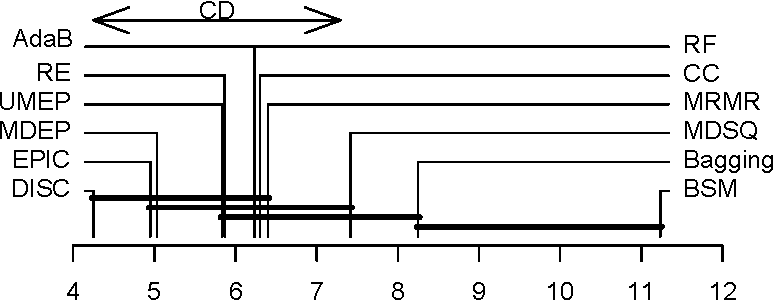
\includegraphics[width=.8\textwidth]{6_analysis/fig/Nemenyi.pdf}
\caption{Comparison of the different metrics over the 30 datasets using the Nemenyi test. Methods not significantly different ($\alpha$=0.05) are connected together.}
\label{Nemenyi}
\end{figure*}

\subsection{Prediction Consistency} \label{precision.con}
\textbf{To answer} $\pmb{Q_8}$, after statistical analysis and according to the Nemenyi test, we selected \{DISC, EPIC, MDEP, UMEP, AdaB, RF, Bagging, BSM\}, and analyzed the distribution of their prediction accuracy over the 100 executions. Figure \ref{ch6_consprediction} presents the range of the prediction accuracy around the median and how the heuristic metrics realize robust and stable predictions, with less number of internal classifiers, for a set of representative datasets \{\textit{D$_1$, D$_3$, D$_4$, D$_6$, D$_9$, D$_{19}$, D$_{25}$, D$_{28}$}\}. The conclusion is that the ordering metrics are more effective to select a promising subensemble and their behavior reduces the performance variance. 

\begin{figure*}[!ht]
\begin{center}\scriptsize
  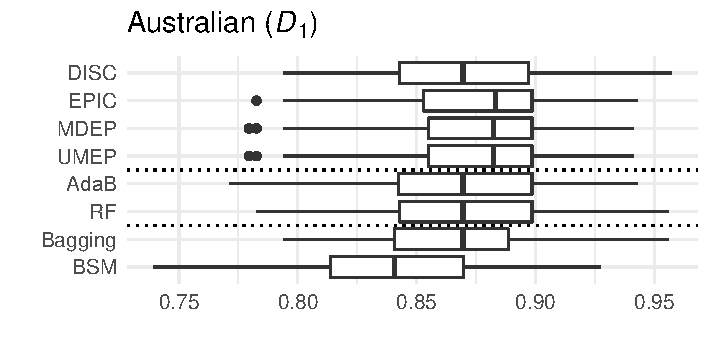
\includegraphics[width=.49\textwidth]{6_analysis/fig/boxplot-Australian.pdf}
  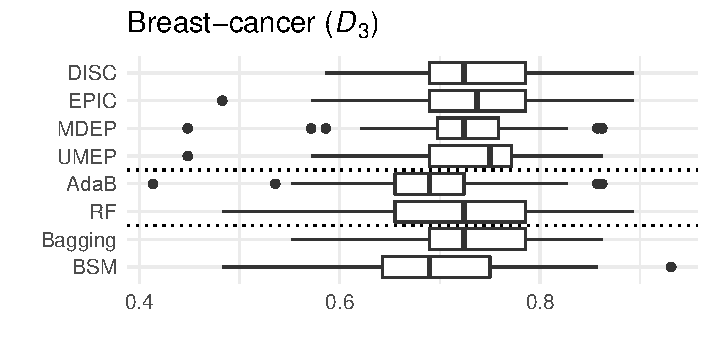
\includegraphics[width=.49\textwidth]{6_analysis/fig/boxplot-Breast-cancer.pdf} \\
  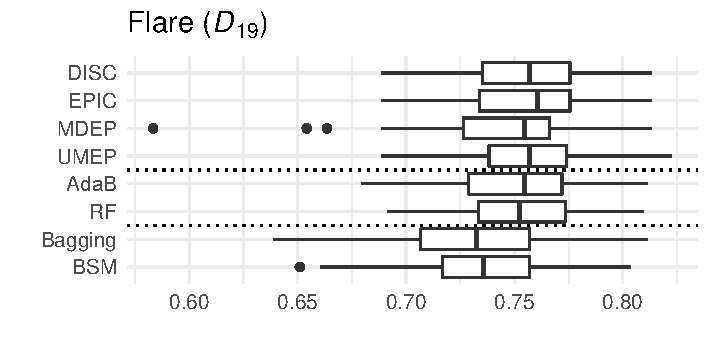
\includegraphics[width=.49\textwidth]{6_analysis/fig/boxplot-Flare.pdf}
  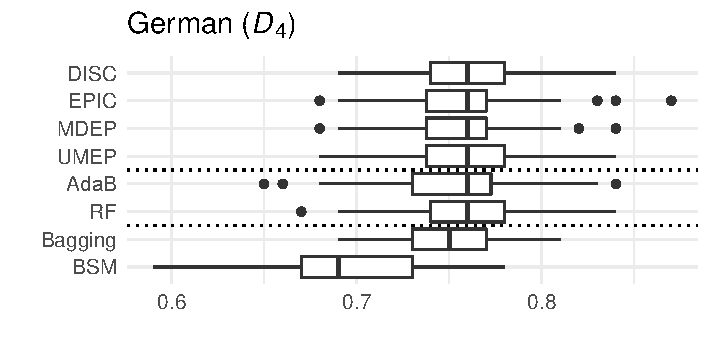
\includegraphics[width=.49\textwidth]{6_analysis/fig/boxplot-German.pdf}\\
  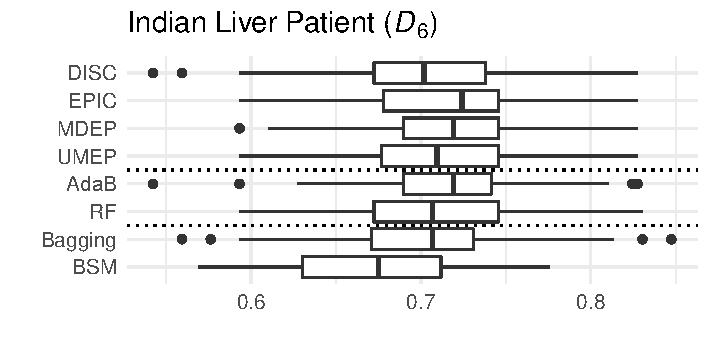
\includegraphics[width=.49\textwidth]{6_analysis/fig/boxplot-Indian Liver Patient.pdf}
  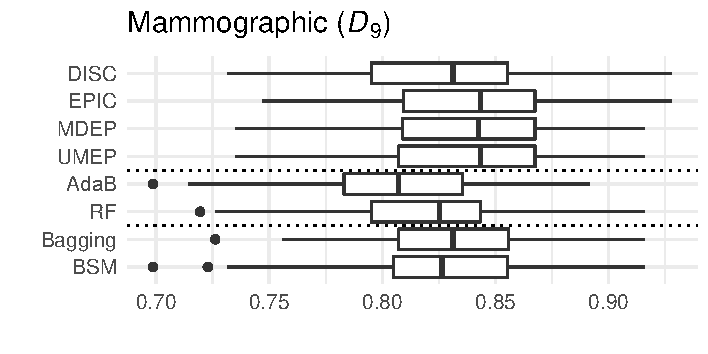
\includegraphics[width=.49\textwidth]{6_analysis/fig/boxplot-Mammographic.pdf}\\
   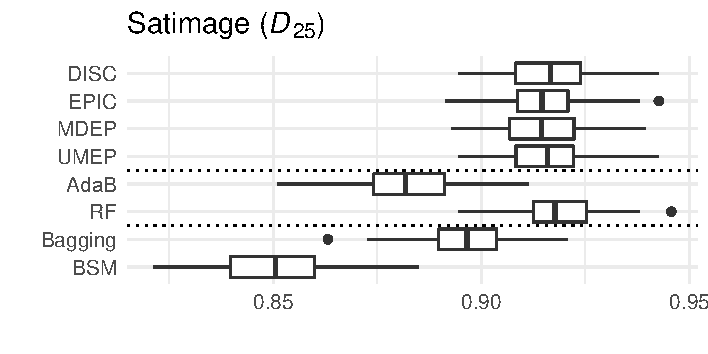
\includegraphics[width=.49\textwidth]{6_analysis/fig/boxplot-Satimage.pdf}
  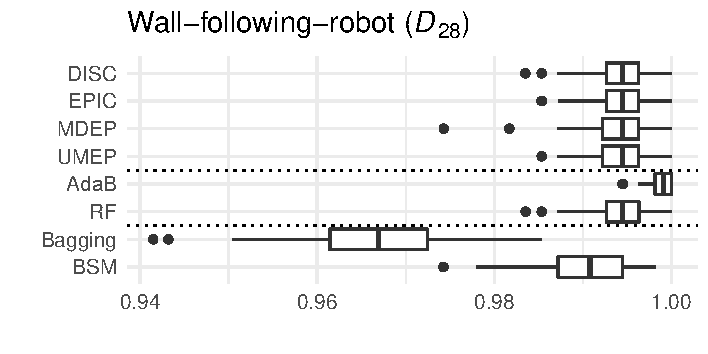
\includegraphics[width=.49\textwidth]{6_analysis/fig/boxplot-Wall-following-robot.pdf}
\end{center}
\caption{Distribution of the prediction accuracy.}
\label{ch6_consprediction}
\end{figure*}


\subsection{Efficiency Analysis } \label{eff.analysis}

As demonstrated in \cite{martinez2009}, the efficiency of reordering metrics can be evaluated according to the following three aspects: the computational cost to extract the pruned subensemble, the required memory space to store the pruned ensembles, and the classification speed.  While, some steps can be performed in parallel: the generation of the initial pool of classifiers, and the retrieving of classification decisions from the selected classifiers.  


\textbf{To answer} $\pmb{Q_9}$, space and time complexities of the different heuristic metrics are summarized in Table \ref{complexity} in terms of $T$, $N$, $M$. The memory requirements are estimated assuming that the decisions of the classifiers are stored in a matrix of size $N \times T$. For large datasets, it might be difficult to store this matrix in memory. In such a case, the whole matrix can be stored to a secondary memory device like the hard disk \cite{martinez2009}. This would reduce the memory requirements to $\mathcal{O}( N )$, but the required disk access will slow down the classification process.   


\begin{table}[!ht]
\centering \scriptsize
 \caption{Space and time complexities of different metrics.}
\label{complexity}
\renewcommand{\arraystretch}{1.3}
\begin{adjustbox}{max width=1\textwidth}
\begin{tabular}{l|l|l}
\hline
Metric & Space complexity & Time complexity\\ \hline
RE& $\mathcal{O}( N \cdot T + M) $ &$\mathcal{O}( T^2 \cdot N \cdot M) $\\
CC& $\mathcal{O}( N \cdot T + M) $ &$\mathcal{O}( T^2 \cdot N) $\\
MDSQ& $\mathcal{O}( N \cdot T ) $ &$\mathcal{O}( T^2 \cdot N) $\\
MRMR& $\mathcal{O}( N \cdot T + M^2)$ &$\mathcal{O}( T^2 \cdot N \cdot M) $\\
DISC& $\mathcal{O}( N \cdot T + M^2)$ &$\mathcal{O}( T^2 \cdot N \cdot M) $\\
EPIC& $\mathcal{O}( N \cdot T + M)$ &$\mathcal{O}(T \cdot N + T \cdot \log{}(T))$\\
UMEP& $\mathcal{O}( N \cdot T ) $ &$\mathcal{O}(T \cdot N+ T \cdot \log{}(T))$\\
MDEP&$\mathcal{O}( N \cdot T + M)$ &$\mathcal{O}(T \cdot N + T \cdot \log{}(T))$\\

\hline
\end{tabular}
\end{adjustbox}
\end{table}




To empirically investigate how the heuristic measures depend on $T$, a series of experiments over the \textit{SPECTF} dataset are performed. Table \ref{time.complexity} presents the execution time of several heterogeneous classifiers with initial bagging of 25, 51, 75, 101, 151, and 201. The values of the remaining parameters are $M=2$, $N_{train}=314$, $D_{pr}=N_{train}$, $P=20\%$. The times are averaged over 100 executions in Intel(R) Core(TM) i5-7200 CPU @ 2.50GHZ with 8 GB of RAM. 

\begin{table}[!ht]
\centering \scriptsize
 \caption{Average execution time in seconds for the \textit{SPECTF} dataset.}
\label{time.complexity}
\renewcommand{\arraystretch}{1.3}
\begin{adjustbox}{max width=1\textwidth}
\begin{tabular}{l|cccccc}
\hline
\diag{.07em}{1.2cm}{Metric}{$T$} & 25 & 51 &75 &101 &151 &201\\  \hline
RE & 0.09 & 0.26 & 0.78 & 1.48 & 3.95 & 5.91\\
CC& 0.06 & 0.26 &	0.68 & 1.20	 & 2.85 & 4.87\\
MDSQ& 0.05 & 0.19 & 0.32 & 0.48 & 1.13 & 2.96\\
MRMR& 0.10 & 0.91 & 1.10 & 2.83 & 4.09 & 7.66\\
DISC& 0.10 & 0.58 & 1.43 & 2.17 & 3.64 &	7.01\\
EPIC& 0.01 & 0.03 & 0.04 & 	0.05 & 0.09 &0.11\\
UMEP& 0.01 & 0.02 & 0.03 & 0.04 & 0.07 & 0.10\\
MDEP& 0.02 & 0.04 & 0.05 & 0.07 & 0.12 & 0.15\\

\hline
\end{tabular}
\end{adjustbox}
\end{table}



The results show that UMEP is the fastest method because the rank is calculated based on the classifier's correct classified samples from the pruning set $D_{pr}$. Additionally, the computation time of EPIC and MDEP is also rather fast with an increasing complexity approximately log-linear with respect to $T$. While, the execution time of RE, CC, MDSQ, MRMR, and DISC is quadratic in $T$. Both MRMR and DISC are much slower, as the selection of one more classifier is conditioned by more internal calculations.       


Besides the efficacy of the ensemble pruning metrics, other main benefits concern the efficiency as; storage requirements and the classification speed. The booked memory space for complete bagging will be released to store the pruned subensemble. While the classification speed depends on both (1) the size of the pruned ensemble and (2) the complexity of the base classifiers. 